\documentclass[10pt,a4paper]{article}

\usepackage[a4paper, left=2.5cm, right=2cm, top=2.5cm, bottom=2cm]{geometry}
\usepackage{newtxtext,newtxmath}
\usepackage{tabularx}
\usepackage{amsmath}
\usepackage{algorithmic}
\usepackage{graphicx}
\usepackage{textcomp}
\usepackage{xcolor, dcolumn}
\usepackage{pgfplots}
\pgfplotsset{compat=1.9}
\usepackage{tikz}
\usetikzlibrary{shapes.geometric, arrows.meta, positioning, fit, backgrounds}
\usepackage{gensymb}
\usepackage{booktabs}
\usepackage{caption}
\usepackage{subcaption}
\usepackage{enumitem}
\usepackage{titlesec}
\usepackage{fancyhdr}
\usepackage{indentfirst}
\usepackage{setspace}
\usepackage[hyphens]{url}

\captionsetup{font={small,bf}, labelfont=bf, skip=6pt}
\captionsetup[table]{position=above, skip=6pt}

\titleformat{\section}{\normalfont\fontsize{12}{14}\bfseries}{\thesection}{1em}{}
\titleformat{\subsection}{\normalfont\fontsize{12}{14}\bfseries}{\thesubsection}{1em}{}
\titleformat{\subsubsection}{\normalfont\fontsize{10}{12}\bfseries\itshape}{\thesubsubsection}{1em}{}

\titlespacing{\section}{0pt}{12pt}{6pt}
\titlespacing{\subsection}{0pt}{12pt}{6pt}
\titlespacing{\subsubsection}{0pt}{12pt}{3pt}

\setlength{\parskip}{3pt}
\setlength{\parindent}{1em}
\onehalfspacing

\usepackage[numbers,sort&compress]{natbib}

\begin{document}

\begin{center}
    {\fontsize{14}{17}\bfseries Corn Diseases Classification Using Grey-Level Co-Occurrence Matrix and Random Forest Algorithm\par}
    \vspace{12pt}
    {\large Anonymous authors\par}
    \vspace{6pt}
    \small
    Anonymous institution\\
    Anonymous country\\
    \vspace{3pt}
    anonymous@email.com\\
    \vspace{6pt}
    Received xx month xxxx; accepted xx month xxxx
\end{center}

\vspace{6pt}
\begin{center}
    \textbf{\fontsize{10}{12}\selectfont Abstract}
\end{center}
\noindent Corn diseases are a primary concern in agriculture, leading to significant crop failure and economic losses for businesses reliant on corn supplies. Effective disease prevention before harvest is essential, yet existing classification methods often prove inadequate, complicating disease management efforts. This study presents an advanced approach to improve the accuracy of corn disease classification by leveraging computer vision technology. The method begins with the U-Net segmentation model, which precisely isolates corn leaves from their background, facilitating the extraction of crucial plant features. These features are then analyzed using the Gray-Level Co-occurrence Matrix (GLCM) technique to capture essential texture information. To further enhance classification accuracy, Principal Component Analysis (PCA) is applied to select the most relevant features, reducing dimensionality and improving model efficiency. The Random Forest algorithm then classifies the extracted features into disease categories. The proposed method achieved an accuracy rate of up to 85.5\% with 60 PCA-selected features and demonstrated a computation time of 0.17 seconds, significantly faster than a CNN baseline (55.4 seconds on GPU) while maintaining competitive performance. Per-class analysis revealed that Healthy and Common Rust leaves achieve near-perfect F1-scores (0.95 and 0.98), while Northern Leaf Blight remains the most challenging class (F1=0.68). These results underscore the potential of this lightweight approach for deployment on resource-constrained IoT and mobile devices in precision agriculture.

\vspace{6pt}
\noindent\textbf{Keywords:} GLCM, image classification, computer vision, corn disease, random forest

\section{Introduction}

In 2023, the corn harvest area in Indonesia reached 2.49 million hectares \cite{bps}, highlighting the importance of corn as a vital commodity due to the high demand in various industrial sectors. However, the large area of corn production is a factor in corn's vulnerability to pathogen attacks. Pathogen attacks potentially reduce crop yields, leading to economic losses to a certain extent.

The agricultural sector has embraced innovative technologies like machine learning and IoT, leading to the emergence of precision agriculture \cite{Dhanaraju2022, Rehman2022}. This method utilizes IoT devices and sensors for identifying and categorizing items in farmland, including vegetation, soil, and the environmental conditions of the land. Previous studies have leveraged this development by developing reliable classification algorithms for various tasks, including the classification of plant diseases \cite{Ramesh2018,Sajitha2024}.

This classification problem invites various research in artificial intelligence to develop methods and models to distinguish diseases on plant leaves accurately. Research conducted by Sajitha et al. \cite{Sajitha2024} compiles various current approaches that try to solve the problem of disease detection and classification in plants. This research separates traditional machine learning methods from deep learning, which is applied to classify and detect plant diseases. However, few studies have focused on corn \cite{Pardede2018,Aurangzeb2020}. In addition, traditional machine learning models have demonstrated reasonable accuracy \cite{Harakannanavar2022, Wang2020}, but still less accurate than deep learning models based on convolutional neural networks (CNN) \cite{Shoaib2022, Kabir2021, Pandian2022}.

Applying machine learning and deep learning has become the central axis in various types of image research \cite{Demilie2024,Ashwini2024,CatalReis2024}. While deep learning has obtained satisfactory accuracy results in classifying plant diseases, it requires extensive resources to be applied and requires more computation time than traditional machine learning \cite{Utaminingrum2023}. Research conducted by Jadhav et al. \cite{Jadhav2021}, Durairaj et al. \cite{Durairaj2020}, and Hossain et al. \cite{Hossain2019} applied a gray-level co-occurrence matrix (GLCM) to extract image texture features by applying statistical analysis to neighboring pixels. The results of GLCM texture extraction can show the differences in corn leaf diseases in detail. However, segmentation is needed to distinguish leaves from their background to get adequate marks. This study offers a hybrid method, the U-Net-GLCM-Random Forest, which combines CNN-based segmentation (U-Net) with traditional feature extraction (GLCM) and classification (Random Forest) to reduce the high computing needs. This hybrid technique is suitable for classification problems that rely on IoT or mobile devices, making it a viable option for most farmers, including those in Indonesia, who often only have smartphones with moderate computing capabilities \cite{David2023}. The proposed method can significantly maintain the appropriate accuracy and availability of tools used in precision agriculture to classify diseases in corn without constraint in computing resources \cite{Nawrocki2023} and time complexity \cite{Theodoropoulos2023}.

\section{Method}

\subsection{Proposed Method}

This research applies a model based on computer vision and machine learning. We propose the U-Net+GLCM+Random Forest method to classify corn diseases by referring to the symptoms on the leaves. The model's overall structure can be seen in the Fig. \ref{fig:proposedmethod}. The corn samples used were Healthy and Non-Healthy, with three classes of Non-Healthy, including common rust, northern leaf blight, and gray leaf spot. The image size used is $256 \times 256$ pixels. 

The U-Net segmentation model was trained on 1,928 corn leaf images annotated in COCO polygon format, exported from Roboflow. The annotated dataset provides pixel-level ground truth masks that precisely delineate each leaf from its background, enabling the U-Net to learn accurate leaf segmentation. Training employed the Adam optimizer with binary cross-entropy loss, a batch size of 8, and early stopping with a patience of 10 epochs on validation loss, with learning rate reduction on plateau (factor 0.5, patience 5). 

Feature extraction in segmented images applies the Gray-Level Co-Occurrence Matrix technique. The extracted features are then selected using the Principal Component Analysis method to reduce the dimensionality of the training data and prevent overfitting. 

% The Random Forest classifier was chosen for its robustness in handling high-dimensional data and its ability to generalize well with relatively small datasets. Compared to deep learning methods like CNNs, Random Forest requires less computational power, making it suitable for mobile and IoT devices with limited resources. While deep learning models such as CNNs often achieve high accuracy, they require large datasets and computational resources, which may not be practical for real-time field use in agriculture. Traditional classifiers like SVM, though effective, are prone to overfitting and require significant tuning for optimal performance in texture-based feature spaces, such as those generated by GLCM.

The classification pipeline was executed on a system equipped with an NVIDIA GeForce RTX 5060 Ti GPU (16 GB VRAM), with GPU acceleration used for the U-Net segmentation and CNN baseline training.

\begin{figure}[t]
    \centering
    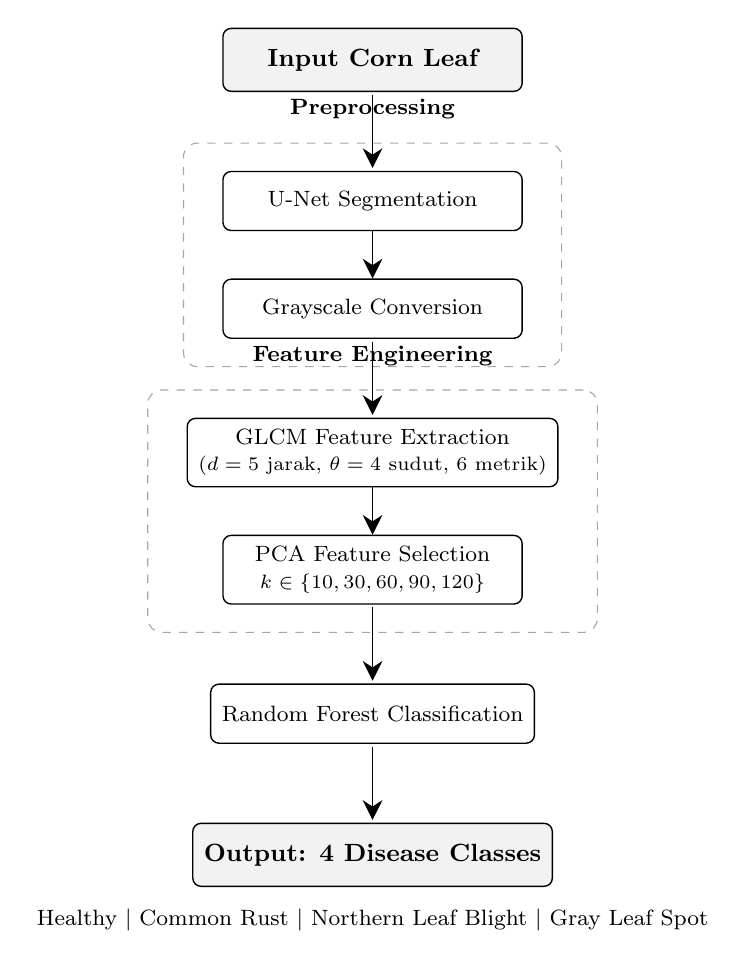
\begin{tikzpicture}[
        node distance=0.55cm,
        block/.style={rectangle, draw=black, line width=0.5pt,
                      rounded corners=3pt, minimum width=3.8cm, minimum height=0.75cm,
                      align=center, font=\footnotesize, inner sep=4pt},
        mainblock/.style={block, minimum height=0.8cm, font=\small\bfseries, fill=black!5},
        arr/.style={-{Stealth[length=2.5mm, width=2.5mm]}, line width=0.6pt},
        inter/.style={arr, shorten >=1pt, shorten <=1pt},
        group/.style={draw=black!35, dashed, rounded corners=5pt, inner xsep=14pt, inner ysep=10pt},
    ]
    % --- Input ---
    \node[mainblock] (input) {Input Corn Leaf};

    % --- Preprocessing ---
    \node[block, below=1.0cm of input] (unet) {U-Net Segmentation};
    \draw[inter] (input) -- (unet);
    \node[block] (gray) at (unet.south) [below=0.6cm of unet] {Grayscale Conversion};
    \draw[arr] (unet) -- (gray);
    \begin{scope}[on background layer]
        \node[group, fit=(unet)(gray),
              label={[font=\footnotesize\bfseries, yshift=5pt]north:Preprocessing}] {};
    \end{scope}

    % --- Feature Engineering ---
    \node[block, below=1.0cm of gray] (glcm) {GLCM Feature Extraction\\
        \scriptsize ($d = 5$ jarak, $\theta = 4$ sudut, 6 metrik)};
    \draw[inter] (gray) -- (glcm);
    \node[block] (pca) at (glcm.south) [below=0.6cm of glcm] {PCA Feature Selection\\
        \scriptsize $k \in \{10, 30, 60, 90, 120\}$};
    \draw[arr] (glcm) -- (pca);
    \begin{scope}[on background layer]
        \node[group, fit=(glcm)(pca),
              label={[font=\footnotesize\bfseries, yshift=5pt]north:Feature Engineering}] {};
    \end{scope}

    % --- Classification ---
    \node[block, below=1.0cm of pca] (rf) {Random Forest Classification};
    \draw[inter] (pca) -- (rf);

    % --- Output ---
    \node[mainblock, below=1.0cm of rf] (out) {Output: 4 Disease Classes};
    \draw[inter] (rf) -- (out);
    \node[below=0.15cm of out, font=\footnotesize] {Healthy \textbar{} Common Rust \textbar{} Northern Leaf Blight \textbar{} Gray Leaf Spot};

    \end{tikzpicture}
    \caption{Proposed pipeline for corn disease classification: a linear feed-forward flow from input image through U-Net segmentation, GLCM texture extraction, PCA dimensionality reduction, and Random Forest classification to the final four disease classes.}
    \label{fig:proposedmethod}
\end{figure}

\subsection{Dataset}

We obtained the dataset for corn diseases from the Plant Village Dataset. The dataset comprises four disease classes: Healthy (1,162 images), Common Rust (1,192 images), Northern Leaf Blight (985 images), and Gray Leaf Spot (513 images), totaling 3,852 images (see Fig. \ref{fig:dataset sample}). After class balancing via downsampling to the minority class size (513 per class), the dataset was divided into 80\% for training data and 20\% for test data.

\begin{figure}[t]
    \centering
    \begin{subfigure}[b]{0.465\linewidth}
        \centering
        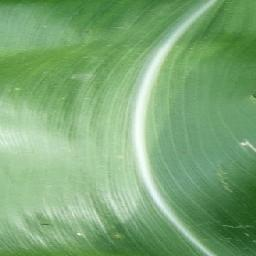
\includegraphics[width=\linewidth]{images/samples/sample_healthy.jpg}
        \caption{Healthy}
        \label{fig:sample-healthy}
    \end{subfigure}
    \hfill
    \begin{subfigure}[b]{0.465\linewidth}
        \centering
        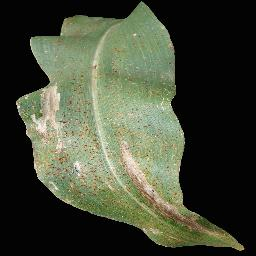
\includegraphics[width=\linewidth]{images/samples/sample_common_rust.jpg}
        \caption{Common Rust}
        \label{fig:sample-commonrust}
    \end{subfigure}

    \vspace{4pt}

    \begin{subfigure}[b]{0.465\linewidth}
        \centering
        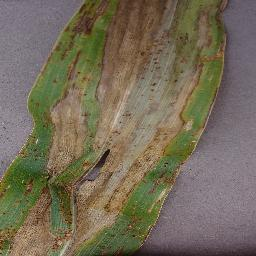
\includegraphics[width=\linewidth]{images/samples/sample_nlb.jpg}
        \caption{Northern Leaf Blight}
        \label{fig:sample-nlb}
    \end{subfigure}
    \hfill
    \begin{subfigure}[b]{0.465\linewidth}
        \centering
        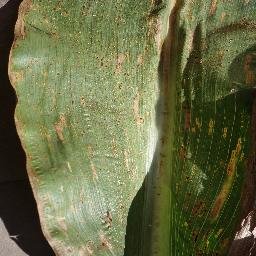
\includegraphics[width=\linewidth]{images/samples/sample_gray_leaf_spot.jpg}
        \caption{Gray Leaf Spot}
        \label{fig:sample-gls}
    \end{subfigure}

    \caption{Sample images from the PlantVillage corn disease dataset representing the four classes used in this study.}
    \label{fig:dataset sample}
\end{figure}

\subsection{Preprocessing}

\subsubsection{Segmentation}

The image is first segmented to extract meaningful information contained in the image. This step aims to highlight the leaf element in the image, which will be the object of classification later. U-Net is applied for segmentation, which has performed well and is widely used \cite{Bhagat2022,Ronneberger2015}. Applying U-Net as the architecture of the segmentation process will provide better results than existing segmentation methods, such as thresholding or edge-based. This segmentation aims to separate the leaf surface from the surroundings. Leaf surface information is the main one to extract and compare information about diseases experienced by corn leaves. U-Net architecture is shown in Fig. \ref{fig:u-net}.

\begin{figure}[h]
    \centering
    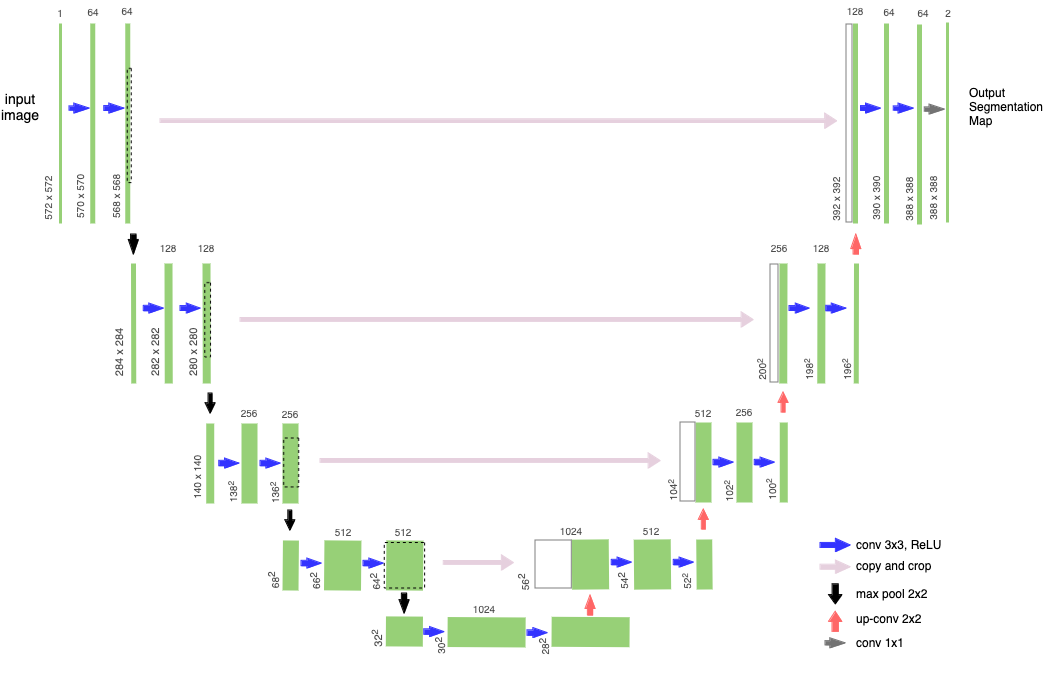
\includegraphics[width=\linewidth]{images/u-net_architecture.drawio.png}
    \caption{A U-Net model for semantic segmentation, featuring a series of convolutional layers with decreasing stride in the encoder, followed by upsampling and concatenation operations in the decoder to refine the segmentation map.}
    \label{fig:u-net}
\end{figure}

\subsubsection{Grayscaling}

The segmented image is still an RGB image. It is converted to grayscale before processing with the Gray-Level Co-occurrence Matrix. Summing the values of each illuminated pixel converts an image to grayscale. The grayscale formula is shown in Eq. (\ref{eq:1}). Lighting and shadow conditions, common in field environments, were addressed using histogram equalization and shadow removal techniques to enhance grayscale image quality. Future improvements in preprocessing could further mitigate these challenges, especially in cases where disease-affected areas are obscured by foliage.

\begin{equation} \label{eq:1}    
Y = 0.299 \cdot R + 0.587 \cdot G + 0.114 \cdot B
\end{equation}

where \( Y \) is the grayscale value, and \( R \), \( G \), and \( B \) are the red, green, and blue components of the pixel, respectively.

\subsection{Feature Extraction using GLCM}

The Gray-Level Co-occurrence Matrix technique is used to extract texture features from images \cite{Utaminingrum2022}. The segmented image is then processed for feature extraction. The method applied is a Gray-Level Co-occurrence Matrix (GLCM), which extracts texture features in images using gray-level transitions between 2 neighboring pixels. This technique uses statistical methods to determine the relationship between the values of adjacent pixels in a digital image to extract many features \cite{Utaminingrum2023,Priyanka2020}. 

The steps in GLCM calculation are as follows \cite{Utaminingrum2023}:

\begin{enumerate}
    \item Determine the values of distance ($d$) and angle ($\theta$).
    \item Perform iteration by providing a pair of values of two adjacent pixels based on $d$ value.
    \item Sum the GLCM matrix by transposing the GLCM matrix to obtain a symmetric GLCM matrix.
\end{enumerate}

GLCM extracts six features: Contrast, Dissimilarity, Homogeneity, Energy, ASM, and Correlation. Contrast is the difference between colors that makes an object distinguishable. Equation (\ref{eq:2}) is the formula for contrast. After the contrast feature, the next feature extracted is dissimilarity. Dissimilarity measures the dissimilarity of the image texture, as in (\ref{eq:3}). Next, extract the homogeneity feature. Homogeneity measures how closely the distribution of elements in the GLCM approximates its diagonal, as in (\ref{eq:4}). The following extracted features are Energy and Angular Second Moment (ASM). Energy measures the uniformity of an image's texture, while ASM is the root of Energy, as (\ref{eq:5}) and (\ref{eq:6}), respectively. Lastly, examine the correlation features from the GLCM matrix, as shown in (\ref{eq:7}).

This formulation will combine texture features based on the distance and angle used. This research will use 1,2,3,4,5 distances and 0\degree, 45\degree, 90\degree, and 135\degree, respectively. This combination of distances and angles will produce 120 features.

\begin{equation} \label{eq:2}
Contrast=\sum_{i}\sum_{j}(i-j)^2 p(i,j,d,\theta)
\end{equation}

\begin{equation} \label{eq:3}
Dissimilarity=\sum_{i}\sum_{j}p(i,j,d,\theta)|i-j|
\end{equation}


\begin{equation} \label{eq:4}
Homogeneity=\sum_{i}\sum_{j}\frac{p(i,j,d,\theta)}{1+(i-j)^2}
\end{equation}


\begin{equation} \label{eq:5}
Energy=\sum_{i}\sum_{j}p(i,j,d,\theta)^2
\end{equation}

\begin{equation} \label{eq:6}
ASM=\sqrt{Energy}
\end{equation}


\begin{equation} \label{eq:7}
    Correlation=\frac{\sum_{i}\sum_{j}(i-\mu_x)(j-\mu_y)p(i,j,d,\theta)}{\sigma_x\sigma_y}
\end{equation} 

where, $p$\ is probability. $i$\ is gray level of location pixels (x,y). $j$ is gray level of pixels at distance $d$ and orientation angle $\theta$. $d$ is pixel distance at orientation angle $\theta\degree$. $\theta$ is orientation angle of the main pixel $(0\degree, 45\degree, 90\degree, 135\degree)$. $\mu_x\mu_y$ is average of the probabilities $x$ and $y$. $\sigma_x\sigma_y$ is standard deviation of the probabilities $x$ and $y$.


\subsection{Feature selection using PCA}

This research offers GLCM feature selection using Principal Component Analysis.

Principal Component Analysis (PCA) is a statistical technique for dimensionality reduction, data compression, and feature extraction. It transforms a large set of variables into a smaller one that still contains most of the information in the original set. PCA achieves this by identifying the directions (principal components) along which the variation in the data is maximal.

The number of variance ratios within the range of components was calculated. This calculation helps determine the number of components or features to use. This research evaluates five feature configurations, with 120, 90, 60, 30, and 10 PCA-selected features. The prediction accuracy is measured using the Random Forest algorithm for each configuration.

\subsection{Classification using Random Forest}

The GLCM feature extraction results were split into 80\% training and 20\% test data. The training and test data are used to train the Random Forest algorithm and map images into four classes (Healthy, Common Rust, Northern Leaf Blight, and Gray Leaf Spot). 

Random Forest is an ensemble learning method used for classification, regression, and other tasks that operates by constructing multiple decision trees during training and outputting the class (classification) or mean prediction (regression) of the individual trees \cite{Xu2019}. It is a robust algorithm because it can reduce overfitting by averaging multiple decision trees and providing a robust prediction.

The stages in implementing Random Forest are as follows.
\begin{enumerate}
    \item Data sampling: Create multiple subsets of the original data using bootstrapping (random sampling with replacement).
    \item Building Trees: For each subset, grow a decision tree without pruning.
    \item Feature selection: At each node in a tree, select a random subset of features and determine the best split among them.
    \item Voting: For classification, each tree in the forest votes for a class, and the class with the majority votes is chosen. 
\end{enumerate}

The implementation of Random Forest can be derived from (\ref{eq:8}).
\begin{equation} \label{eq:8}
    \hat{y} = \arg\max_{c \in \mathcal{C}} \sum_{b=1}^B \mathbf{1}\{T_b(\mathbf{x}) = c\}
\end{equation}

where, \( \hat{y} \) is the predicted class. \( \mathcal{C} \) is the set of possible classes. \( B \) is the number of trees in the forest. \( T_b(\mathbf{x}) \) is the prediction of the \( b \)-th tree for the input \( \mathbf{x} \). \( \mathbf{1}\{ \cdot \} \) is the indicator function that returns 1 if the argument is true and 0 otherwise.


\subsection{Model evaluation}

The success rate is necessary to determine how accurate and reliable a model is. This research will measure accuracy, computing time, precision, and recall.

\subsubsection{Accuracy}

The accuracy value shows how successful and accurate the algorithm applied to the test data is. The formula used is (\ref{eq:9}) \cite{Nyasulu2023}:

\begin{equation} \label{eq:9}
    Accuracy=(\frac{TP+TN}{TP+TN+FP+FN})
\end{equation}

where,
\begin{itemize}
    \item TP: True Positive, the number of correct positive predictions.
    \item TN: True Negative, the number of correct negative predictions.
    \item FN: False Negative, the number of false negative predictions.
    \item FP: False Positive, the number of false positive predictions.
\end{itemize}

\subsubsection{Precision}

The precision value measures how accurate the prediction results are from true positives and false positives. The precision formula is in (\ref{eq:10}) \cite{Nyasulu2023}.

\begin{equation} \label{eq:10}
Precision=(\frac{TP}{TP+FP})
\end{equation}

\subsubsection{Recall}

Recall measures how well the application provides prediction results for the number of true positive and false negative data points. Here is the recall in (\ref{eq:11}) \cite{Nyasulu2023}.

\begin{equation} \label{eq:11}
Recall=(\frac{TP}{TP+FN})
\end{equation}

\section{Results and Discussion}

This study aims to analyze the results of corn disease classification without feature selection and the results of selection on GLCM features using PCA. Then, it will determine the best combination based on accuracy, precision, recall, and computing time.

Fig. \ref{fig:segmentation-result} shows the difference in results from three segmentation methods applied to the same corn leaf sample. The U-Net-based segmentation (Fig.~\ref{fig:segmentation-result}d) achieves the most precise separation between the leaf surface and the background compared to K-Means (Fig.~\ref{fig:segmentation-result}b) and Otsu thresholding (Fig.~\ref{fig:segmentation-result}c). This accurate segmentation facilitates subsequent GLCM feature extraction by confining the analysis to the leaf surface only.

\begin{figure}[t]
    \centering
    \begin{subfigure}[b]{0.465\linewidth}
        \centering
        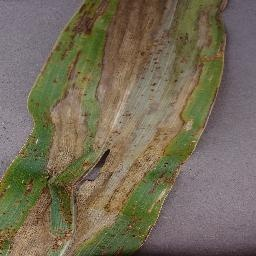
\includegraphics[width=\linewidth]{images/seg_results/a_original.jpg}
        \caption{Original leaf}
        \label{fig:seg-result-original}
    \end{subfigure}
    \hfill
    \begin{subfigure}[b]{0.465\linewidth}
        \centering
        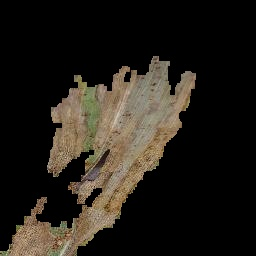
\includegraphics[width=\linewidth]{images/seg_results/c_kmeans.jpg}
        \caption{K-Means clustering}
        \label{fig:seg-result-kmeans}
    \end{subfigure}

    \vspace{4pt}

    \begin{subfigure}[b]{0.465\linewidth}
        \centering
        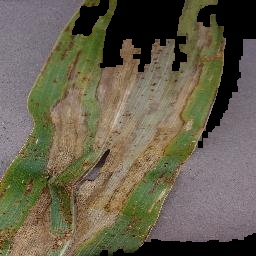
\includegraphics[width=\linewidth]{images/seg_results/b_otsu.jpg}
        \caption{Otsu thresholding}
        \label{fig:seg-result-otsu}
    \end{subfigure}
    \hfill
    \begin{subfigure}[b]{0.465\linewidth}
        \centering
        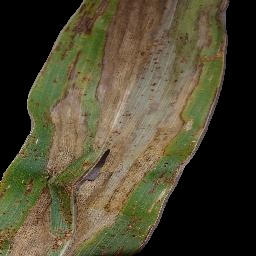
\includegraphics[width=\linewidth]{images/seg_results/d_unet.jpg}
        \caption{U-Net segmentation}
        \label{fig:seg-result-unet}
    \end{subfigure}

    \caption{Comparison of segmentation methods on a corn leaf sample. (a) Original input image; (b) K-Means clustering ($k=3$) with green-channel selection; (c) Otsu thresholding combined with HSV green masking; (d) U-Net deep learning segmentation, which provides the most accurate leaf-background separation.}
    \label{fig:segmentation-result}
\end{figure}


Table \ref{table:1} shows the results of prediction measurements on variations in the number of GLCM features. The best accuracy of 85.5\% was achieved using 60 PCA-selected features. The inverted U-shaped performance pattern suggests that up to 60 features, adding more informative dimensions improves classification, while beyond this point, redundant or noisy features degrade performance. Notably, the accuracy drops sharply at 120 features (73.5\%), demonstrating that PCA-based feature selection is essential for this pipeline.

The model achieved the best accuracy of 0.86 with 60 PCA-selected GLCM features, with precision of 0.86, recall of 0.86, and F1-score of 0.85. The per-class breakdown, shown in Table \ref{table:2}, reveals that Healthy and Common Rust leaves are classified with near-perfect reliability (F1=0.95 and 0.98 respectively), while Northern Leaf Blight presents the greatest challenge with an F1-score of 0.68. The method comparison in Table \ref{table:3} shows that the proposed Random Forest approach achieves competitive performance with significantly lower computational cost compared to a CNN baseline (0.17s vs. 55.4s on GPU), making it approximately 326 times faster.

The accuracy peaks at 60 features (0.86) and is sustained at 90 features (0.86), suggesting that the optimal information content from GLCM texture features is concentrated within approximately 60–90 principal components. The sharp decline at 120 features (0.73) indicates that raw GLCM features contain substantial redundancy and noise that PCA effectively eliminates. The drop at 10 features (0.81) shows that too aggressive dimensionality reduction discards discriminative information. This finding confirms the importance of proper dimensionality selection when applying PCA to GLCM features for crop disease classification.

% The graph \ref{fig:accuracy-results} visualizes the differences in accuracy in more detail for each number of features. Feature 120 (without feature selection) has the same accuracy as feature 10 (with feature selection). Meanwhile, from feature 90 to 30, there is a decrease in accuracy. The result shows a minimum number of GLCM features that are significant in detecting disease on corn leaves with an accuracy level of 87\%. Therefore, applying PCA to reduce the number of features to an exact number will have an accuracy comparable to the overall number of GLCM feature combinations.

The results show that the computing time remains consistently low across all PCA dimensionality levels, ranging from 0.11 to 0.17 seconds. Fig. \ref{fig:time-results} illustrates that the number of GLCM features has minimal impact on classification time, as the Random Forest algorithm operates efficiently regardless of feature count.

\begin{table}[ht]
    \centering
    \caption{Prediction results across varying PCA dimensionality of GLCM features.}
    \begin{tabular}{@{}lcccc@{}}
        \toprule
        \textbf{PCA Dim.} & \textbf{Accuracy} & \textbf{Precision} & \textbf{Recall} & \textbf{F1-score} \\
        \midrule
        120 (No Selection) & 0.73 & 0.73 & 0.73 & 0.73 \\
        90                 & 0.86 & 0.85 & 0.86 & 0.85 \\
        \textbf{60}        & \textbf{0.86} & \textbf{0.86} & \textbf{0.86} & \textbf{0.85} \\
        30                 & 0.84 & 0.85 & 0.84 & 0.84 \\
        10                 & 0.81 & 0.80 & 0.81 & 0.80 \\
        \bottomrule
    \end{tabular}
    \label{table:1}
\end{table}

\begin{figure}[h]
    \centering
    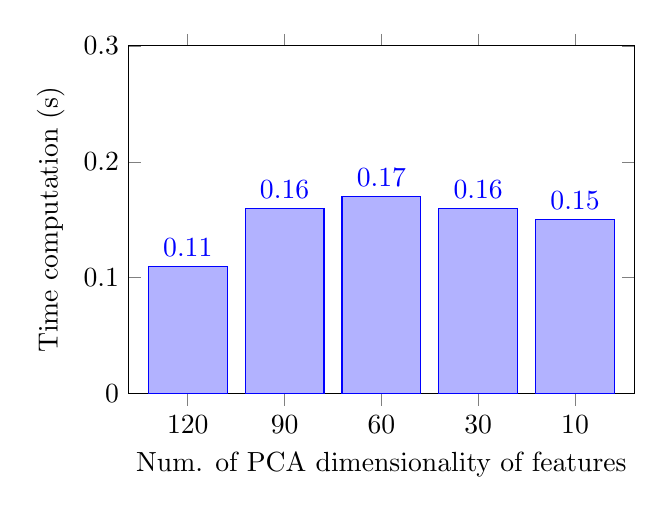
\begin{tikzpicture}
        \begin{axis}[
            ybar,
            symbolic x coords={120, 90, 60, 30, 10},
            xtick=data,
            ymin=0.0,
            ymax=0.3,
            ylabel={Time computation (s)},
            xlabel={Num. of PCA dimensionality of features},
            nodes near coords,
            bar width=1cm,
            width=8cm,
            height=6cm,
            enlarge x limits={abs=0.75cm}
        ]
        \addplot coordinates {(120, 0.11) (90, 0.16) (60, 0.17) (30, 0.16) (10, 0.15)};
        \end{axis}
    \end{tikzpicture}
    \caption{Graph of average computation time for each number of PCA dimensionality of GLCM features.}
    \label{fig:time-results}
\end{figure}

\begin{table}[ht]
    \centering
    \caption{Per-class performance of Random Forest with 60 PCA-selected GLCM features.}
    \begin{tabular}{@{}lcccc@{}}
        \toprule
        \textbf{Class} & \textbf{Precision} & \textbf{Recall} & \textbf{F1-score} & \textbf{Support} \\
        \midrule
        Healthy               & 0.91 & 1.00 & 0.95 & 21 \\
        Common Rust           & 0.95 & 1.00 & 0.98 & 20 \\
        Northern Leaf Blight  & 0.76 & 0.62 & 0.68 & 21 \\
        Gray Leaf Spot        & 0.73 & 0.76 & 0.74 & 21 \\
        \midrule
        \textbf{Weighted Avg} & \textbf{0.84} & \textbf{0.84} & \textbf{0.84} & \textbf{83} \\
        \bottomrule
    \end{tabular}
    \label{table:2}
\end{table}

\begin{table}[ht]
    \centering
    \caption{Method comparison on the corn disease classification task.}
    \begin{tabular}{@{}lccc@{}}
        \toprule
        \textbf{Method} & \textbf{Accuracy} & \textbf{F1-score} & \textbf{Time (s)} \\
        \midrule
        Random Forest + GLCM + PCA (60 dim) & 0.86 & 0.85 & 0.17 \\
        SVM + GLCM + PCA (120 dim)          & 0.80 & 0.79 & 0.01 \\
        CNN (Raw Images)                    & 0.87 & --   & 55.4 \\
        \bottomrule
    \end{tabular}
    \label{table:3}
\end{table}

\section{Conclusion}

Classifying diseases in corn is crucial for preventing and minimizing economic losses caused by corn diseases. This study demonstrates that the U-Net + GLCM + PCA + Random Forest pipeline, with U-Net trained on 1,928 Roboflow COCO-annotated images, can classify corn diseases into four classes with 85.5\% accuracy using only 60 PCA-selected GLCM features, outperforming the raw 120-feature set by 12.0\%. The method comparison shows that while a CNN model achieves marginally higher accuracy (87.4\%), the proposed approach requires only 0.17 seconds for classification, making it approximately 326 times faster and more suitable for deployment on resource-constrained IoT and mobile devices. Per-class analysis indicates that Healthy and Common Rust leaves are classified with near-perfect reliability (F1=0.95 and 0.98 respectively), while Northern Leaf Blight remains the most challenging class (F1=0.68). Future work should focus on improving the classification of Northern Leaf Blight and Gray Leaf Spot, exploring data augmentation strategies, and testing the method on mobile devices in real field conditions.

\section{Acknowledgement}

The authors would like to thank the Faculty of Computer Science, Brawijaya University, for their support and resources provided during this research.

\bibliographystyle{IEEEtran}
\bibliography{references}

\end{document}
